% ============================================================
\chapter{R\'eseaux de Neurones sur Graphes}
\label{ch:gnn}
% ============================================================

Les r\'eseaux de neurones convolutifs ont r\'evolutionn\'e la vision par ordinateur, mais ils reposent sur une hypoth\`ese implicite~: les donn\'ees vivent sur une grille r\'eguli\`ere. Que faire lorsque les donn\'ees sont un r\'eseau social, une mol\'ecule, un maillage 3D ou un r\'eseau de transport~? Ces structures sont naturellement repr\'esent\'ees par des \emph{graphes}, o\`u la notion de voisinage est irr\'eguli\`ere et variable. L'id\'ee des \emph{Graph Neural Networks} (GNN), formalis\'ee par Franco Scarselli en 2009 puis red\'ecouverte et \'etendue par Thomas Kipf, Petar Veli\v{c}kovi\'c et bien d'autres \`a partir de 2016, est d'adapter le m\'ecanisme de convolution \`a cette g\'eom\'etrie irr\'eguli\`ere~: chaque n\oe ud met \`a jour sa repr\'esentation en agr\'egeant les messages de ses voisins.

Ce paradigme de \emph{passage de messages} est devenu le cadre unificateur de l'apprentissage sur graphes. Ce chapitre en construit les fondations.

\section{Repr\'esentation des graphes}

\begin{definition}[Graphe attribu\'e]
Un \textbf{graphe attribu\'e} est un tuple $G = (V, E, \mathbf{X}, \mathbf{E})$ o\`u~:
\begin{itemize}
    \item $V = \{1, \ldots, n\}$ est l'ensemble des \textbf{n\oe uds}.
    \item $E \subseteq V \times V$ est l'ensemble des \textbf{ar\^etes}.
    \item $\mathbf{X} \in \R^{n \times d}$ est la matrice des \textbf{attributs de n\oe uds}.
    \item $\mathbf{E} \in \R^{\abs{E} \times d_e}$ contient les \textbf{attributs d'ar\^etes}.
\end{itemize}
\end{definition}

\begin{definition}[Matrices associ\'ees]
Pour un graphe $G = (V, E)$~:
\begin{itemize}
    \item \textbf{Matrice d'adjacence}~: $A_{ij} = 1$ si $(i,j) \in E$, $0$ sinon.
    \item \textbf{Matrice des degr\'es}~: $D_{ii} = \sum_j A_{ij}$ (diagonale).
    \item \textbf{Laplacien}~: $\mathbf{L} = \mathbf{D} - \mathbf{A}$.
    \item \textbf{Laplacien normalis\'e}~:
          $\tilde{\mathbf{L}} = \mathbf{I} - \mathbf{D}^{-1/2}\mathbf{A}\mathbf{D}^{-1/2}$.
\end{itemize}
\end{definition}

\begin{codeblock}[title=\textbf{Repr\'esentation de graphes dans PyTorch Geometric}]
\begin{minted}{python}
import torch
from torch_geometric.data import Data

# Graphe avec 4 noeuds et 5 aretes (non dirige)
edge_index = torch.tensor([
    [0, 1, 1, 2, 2, 3, 3, 0, 1, 3],
    [1, 0, 2, 1, 3, 2, 0, 3, 3, 1]
], dtype=torch.long)

# Attributs des noeuds (4 noeuds, 3 attributs)
x = torch.tensor([
    [1.0, 0.0, 0.0],  # noeud 0 : carbone
    [0.0, 1.0, 0.0],  # noeud 1 : azote
    [0.0, 0.0, 1.0],  # noeud 2 : oxygene
    [1.0, 0.0, 0.0],  # noeud 3 : carbone
], dtype=torch.float)

data = Data(x=x, edge_index=edge_index)
print(f"Noeuds: {data.num_nodes}, Aretes: {data.num_edges}")
print(f"Attributs: {data.x.shape}")
print(f"Isole: {data.has_isolated_nodes()}")
print(f"Self-loops: {data.has_self_loops()}")
\end{minted}
\end{codeblock}

\section{Le paradigme du passage de messages}

\subsection{Formalisation g\'en\'erale}

\begin{definition}[R\'eseau de neurones \`a passage de messages (MPNN)]
Un \textbf{MPNN} (Gilmer et al., 2017) met \`a jour les repr\'esentations des
n\oe uds par des it\'erations de la forme~:
\begin{align}
    \mathbf{m}_v^{(\ell+1)} &= \bigoplus_{u \in \mathcal{N}(v)}
    \psi^{(\ell)}\!\left(\mathbf{h}_v^{(\ell)}, \mathbf{h}_u^{(\ell)},
    \mathbf{e}_{uv}\right) \quad \text{(agr\'egation des messages)} \label{eq:mpnn_agg} \\
    \mathbf{h}_v^{(\ell+1)} &= \phi^{(\ell)}\!\left(\mathbf{h}_v^{(\ell)},
    \mathbf{m}_v^{(\ell+1)}\right) \quad \text{(mise \`a jour)} \label{eq:mpnn_upd}
\end{align}
o\`u~:
\begin{itemize}
    \item $\psi^{(\ell)}$ est la \textbf{fonction de message}.
    \item $\bigoplus$ est un op\'erateur d'\textbf{agr\'egation} invariant par
          permutation (somme, moyenne, max).
    \item $\phi^{(\ell)}$ est la \textbf{fonction de mise \`a jour}.
    \item $\mathbf{h}_v^{(0)} = \mathbf{x}_v$ (attributs initiaux).
\end{itemize}
\end{definition}

\begin{theoreme}[\'Equivariance des MPNN]
Toute couche MPNN avec agr\'egation invariante par permutation est
\textbf{\'equivariante par permutation des n\oe uds}~: si $\pi \in S_n$
est une permutation, alors~:
\[
    \mathbf{h}_{\pi(v)}^{(\ell+1)}(\pi \cdot G) = \mathbf{h}_v^{(\ell+1)}(G)
\]
o\`u $\pi \cdot G$ est le graphe avec n\oe uds renum\'erot\'es par $\pi$.
\end{theoreme}

\begin{proof}
L'agr\'egation $\bigoplus$ est invariante par permutation par hypoth\`ese. Les
fonctions $\psi$ et $\phi$ sont appliqu\'ees individuellement \`a chaque n\oe ud.
Le voisinage $\mathcal{N}(\pi(v))$ dans $\pi \cdot G$ est exactement
$\{\pi(u) : u \in \mathcal{N}(v)\}$ dans $G$. Donc~:
\begin{align*}
    \mathbf{m}_{\pi(v)}^{(\ell+1)}(\pi \cdot G)
    &= \bigoplus_{w \in \mathcal{N}(\pi(v))} \psi(\mathbf{h}_{\pi(v)}, \mathbf{h}_w, \mathbf{e}_{w,\pi(v)}) \\
    &= \bigoplus_{u \in \mathcal{N}(v)} \psi(\mathbf{h}_v, \mathbf{h}_u, \mathbf{e}_{uv})
    = \mathbf{m}_v^{(\ell+1)}(G). \qedhere
\end{align*}
\end{proof}

\subsection{Illustration du passage de messages}

\begin{figure}[htbp]
\centering
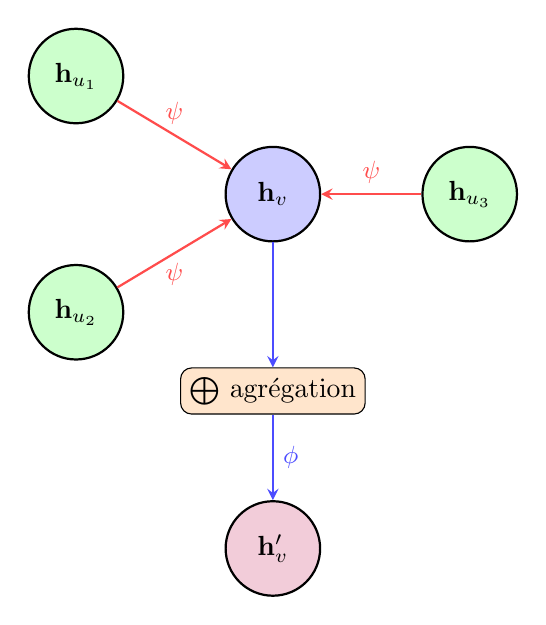
\begin{tikzpicture}[
    node_style/.style={circle, draw, thick, minimum size=12mm, inner sep=0pt},
    msg/.style={->, thick, >=stealth, color=red!70},
    upd/.style={->, thick, >=stealth, color=blue!70}
]
% Graphe
\node[node_style, fill=blue!20] (v) at (0, 0) {$\mathbf{h}_v$};
\node[node_style, fill=green!20] (u1) at (-2.5, 1.5) {$\mathbf{h}_{u_1}$};
\node[node_style, fill=green!20] (u2) at (-2.5, -1.5) {$\mathbf{h}_{u_2}$};
\node[node_style, fill=green!20] (u3) at (2.5, 0) {$\mathbf{h}_{u_3}$};

\draw[msg] (u1) -- node[above, font=\small, color=red!70] {$\psi$} (v);
\draw[msg] (u2) -- node[below, font=\small, color=red!70] {$\psi$} (v);
\draw[msg] (u3) -- node[above, font=\small, color=red!70] {$\psi$} (v);

% Aggregation
\node[rectangle, draw, fill=orange!20, rounded corners] (agg) at (0, -2.5)
    {$\bigoplus$ agr\'egation};
\draw[upd] (v) -- (agg);

% Update
\node[node_style, fill=purple!20] (vnew) at (0, -4.5) {$\mathbf{h}_v'$};
\draw[upd] (agg) -- node[right, font=\small, color=blue!70] {$\phi$} (vnew);
\end{tikzpicture}
\caption{Sch\'ema du passage de messages~: messages, agr\'egation, mise \`a jour.}
\end{figure}

\section{Graph Convolutional Network (GCN)}

\begin{definition}[Couche GCN --- Kipf et Welling, 2017]
La couche GCN utilise la \textbf{r\`egle de propagation} suivante~:
\[
    \mathbf{H}^{(\ell+1)} = \sigma\!\left(\hat{\mathbf{D}}^{-1/2}
    \hat{\mathbf{A}}\, \hat{\mathbf{D}}^{-1/2}\, \mathbf{H}^{(\ell)}\,
    \mathbf{W}^{(\ell)}\right)
\]
o\`u~:
\begin{itemize}
    \item $\hat{\mathbf{A}} = \mathbf{A} + \mathbf{I}$ (ajout de self-loops).
    \item $\hat{\mathbf{D}}_{ii} = \sum_j \hat{A}_{ij}$ (degr\'es ajust\'es).
    \item $\mathbf{W}^{(\ell)} \in \R^{d_\ell \times d_{\ell+1}}$ est la matrice de poids.
    \item $\sigma$ est une activation non lin\'eaire (ReLU).
\end{itemize}
\end{definition}

\begin{remarque}[Interpr\'etation]
Pour un n\oe ud $v$, la couche GCN calcule~:
\[
    \mathbf{h}_v^{(\ell+1)} = \sigma\!\left(\sum_{u \in \mathcal{N}(v) \cup \{v\}}
    \frac{1}{\sqrt{\hat{d}_v \hat{d}_u}}\, \mathbf{h}_u^{(\ell)}\, \mathbf{W}^{(\ell)}\right)
\]
C'est une \textbf{moyenne pond\'er\'ee} des repr\'esentations des voisins, suivie
d'une transformation lin\'eaire et d'une non-lin\'earit\'e.
\end{remarque}

\begin{proposition}[Lien avec le laplacien]
La couche GCN peut s'\'ecrire~:
\[
    \mathbf{H}^{(\ell+1)} = \sigma\!\left((\mathbf{I} - \tilde{\mathbf{L}}_{\text{sym}})
    \mathbf{H}^{(\ell)} \mathbf{W}^{(\ell)}\right)
\]
o\`u $\tilde{\mathbf{L}}_{\text{sym}}$ est le laplacien normalis\'e de $\hat{G}$
(graphe avec self-loops). La couche GCN r\'ealise donc un \textbf{lissage
laplacien} des attributs.
\end{proposition}

\begin{codeblock}[title=\textbf{Impl\'ementation GCN compl\`ete}]
\begin{minted}{python}
import torch
import torch.nn as nn
import torch.nn.functional as F
from torch_geometric.nn import GCNConv, global_mean_pool
from torch_geometric.datasets import Planetoid
from torch_geometric.loader import DataLoader

class GCN(nn.Module):
    def __init__(self, in_channels, hidden_channels, out_channels,
                 num_layers=3, dropout=0.5):
        super().__init__()
        self.convs = nn.ModuleList()
        self.convs.append(GCNConv(in_channels, hidden_channels))
        for _ in range(num_layers - 2):
            self.convs.append(GCNConv(hidden_channels, hidden_channels))
        self.convs.append(GCNConv(hidden_channels, out_channels))
        self.dropout = dropout

    def forward(self, x, edge_index):
        for i, conv in enumerate(self.convs[:-1]):
            x = conv(x, edge_index)
            x = F.relu(x)
            x = F.dropout(x, p=self.dropout, training=self.training)
        x = self.convs[-1](x, edge_index)
        return x

# Classification de noeuds sur Cora
dataset = Planetoid(root='/tmp/Cora', name='Cora')
data = dataset[0]

model = GCN(dataset.num_features, 64, dataset.num_classes)
optimizer = torch.optim.Adam(model.parameters(), lr=0.01, weight_decay=5e-4)

# Entrainement
model.train()
for epoch in range(200):
    optimizer.zero_grad()
    out = model(data.x, data.edge_index)
    loss = F.cross_entropy(out[data.train_mask], data.y[data.train_mask])
    loss.backward()
    optimizer.step()

# Evaluation
model.eval()
pred = model(data.x, data.edge_index).argmax(dim=1)
correct = (pred[data.test_mask] == data.y[data.test_mask]).sum()
acc = correct / data.test_mask.sum()
print(f"Precision test: {acc:.4f}")
\end{minted}
\end{codeblock}

\section{Le probl\`eme du sur-lissage}

\begin{theoreme}[Sur-lissage --- Li et al., 2018]
En empilant $L$ couches GCN, les repr\'esentations de tous les n\oe uds
convergent vers un point fixe~:
\[
    \lim_{L \to \infty} \mathbf{H}^{(L)} = \mathbf{1}\boldsymbol{\pi}^\top \mathbf{H}^{(0)} \mathbf{W}_\infty
\]
o\`u $\boldsymbol{\pi}$ est le vecteur propre dominant du graphe (li\'e \`a
la distribution stationnaire du random walk). Tous les n\oe uds obtiennent
la \textbf{m\^eme repr\'esentation}.
\end{theoreme}

\begin{attention}[title=\textbf{Cons\'equences pratiques}]
\begin{itemize}
    \item Les GNN profonds ($L > 5$) perdent souvent en performance.
    \item Les repr\'esentations deviennent indistinguables entre n\oe uds.
    \item Solutions~: connexions r\'esiduelles, normalisation, DropEdge.
\end{itemize}
\end{attention}

\section{Readout et pr\'ediction au niveau du graphe}

\begin{definition}[Readout]
Pour obtenir une repr\'esentation au niveau du graphe \`a partir des
repr\'esentations de n\oe uds, on utilise une fonction de \textbf{readout}
invariante par permutation~:
\[
    \mathbf{h}_G = \text{READOUT}(\{\mathbf{h}_v^{(L)} : v \in V\})
\]
Options courantes~:
\begin{itemize}
    \item Somme~: $\mathbf{h}_G = \sum_{v \in V} \mathbf{h}_v^{(L)}$
    \item Moyenne~: $\mathbf{h}_G = \frac{1}{\abs{V}} \sum_{v \in V} \mathbf{h}_v^{(L)}$
    \item Max~: $\mathbf{h}_G = \max_{v \in V} \mathbf{h}_v^{(L)}$
    \item Attention~: somme pond\'er\'ee par des poids appris.
\end{itemize}
\end{definition}

\section{Pouvoir expressif des GNN}

\begin{theoreme}[Lien avec le test de Weisfeiler--Leman --- Xu et al., 2019]
Les MPNN sont \textbf{au plus aussi expressifs} que le test de
Weisfeiler--Leman d'ordre 1 (1-WL). Plus pr\'ecis\'ement~:
\begin{enumerate}
    \item Si le 1-WL distingue deux graphes $G_1$ et $G_2$, alors il existe
          un MPNN qui les distingue.
    \item Si le 1-WL ne distingue pas $G_1$ et $G_2$, alors \textbf{aucun}
          MPNN ne les distingue.
\end{enumerate}
\end{theoreme}

\begin{definition}[Test de Weisfeiler--Leman (1-WL)]
Le test 1-WL est un algorithme it\'eratif de raffinement de couleurs~:
\begin{enumerate}
    \item \textbf{Initialisation}~: $c_v^{(0)} = \text{couleur initiale de } v$.
    \item \textbf{It\'eration}~: $c_v^{(t+1)} = \text{HASH}\!\left(c_v^{(t)},
          \{\!\!\{c_u^{(t)} : u \in \mathcal{N}(v)\}\!\!\}\right)$
    \item \textbf{Arr\^et}~: quand les couleurs se stabilisent.
\end{enumerate}
o\`u $\{\!\!\{\cdot\}\!\!\}$ d\'enote un multi-ensemble.
\end{definition}

\begin{figure}[htbp]
\centering
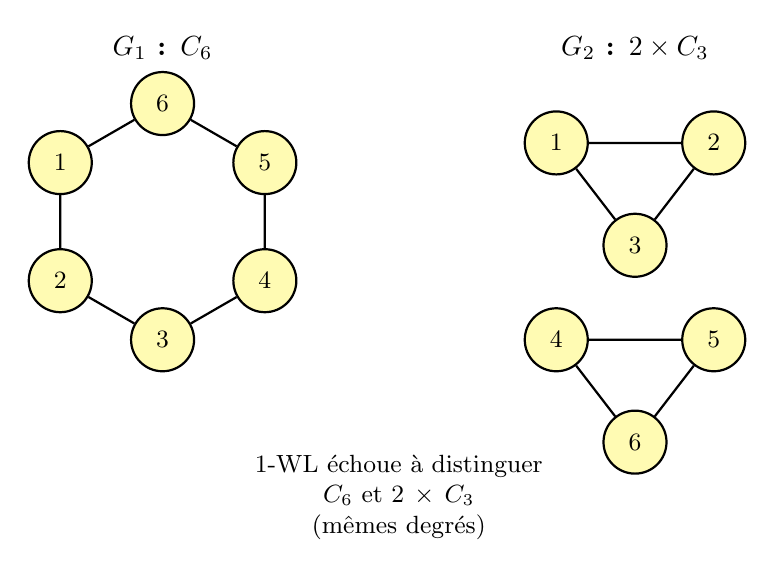
\begin{tikzpicture}[
    node_style/.style={circle, draw, thick, minimum size=8mm, inner sep=0pt, font=\small}
]
% Graphe 1 : cycle C6
\begin{scope}[shift={(-3,0)}]
    \node[font=\bfseries] at (0, 2.2) {$G_1$~: $C_6$};
    \foreach \i in {1,...,6} {
        \pgfmathsetmacro{\angle}{60*\i + 90}
        \node[node_style, fill=yellow!30] (a\i) at (\angle:1.5) {\i};
    }
    \draw[thick] (a1)--(a2)--(a3)--(a4)--(a5)--(a6)--(a1);
\end{scope}
% Graphe 2 : deux triangles
\begin{scope}[shift={(3,0)}]
    \node[font=\bfseries] at (0, 2.2) {$G_2$~: $2 \times C_3$};
    \node[node_style, fill=yellow!30] (b1) at (-1, 1) {1};
    \node[node_style, fill=yellow!30] (b2) at (1, 1) {2};
    \node[node_style, fill=yellow!30] (b3) at (0, -0.3) {3};
    \node[node_style, fill=yellow!30] (b4) at (-1, -1.5) {4};
    \node[node_style, fill=yellow!30] (b5) at (1, -1.5) {5};
    \node[node_style, fill=yellow!30] (b6) at (0, -2.8) {6};
    \draw[thick] (b1)--(b2)--(b3)--(b1);
    \draw[thick] (b4)--(b5)--(b6)--(b4);
\end{scope}
\node[font=\small, text width=4cm, align=center] at (0, -3.5)
    {1-WL \'echoue \`a distinguer\\$C_6$ et $2\times C_3$\\(m\^emes degr\'es)};
\end{tikzpicture}
\caption{Deux graphes r\'eguliers que le 1-WL (et donc les MPNN) ne distinguent pas.}
\end{figure}

\section{GCN \`a la main}

\begin{codeblock}[title=\textbf{GCN impl\'ement\'ee from scratch}]
\begin{minted}{python}
import torch
import torch.nn as nn

class GCNLayerManual(nn.Module):
    """Couche GCN implementee manuellement."""
    def __init__(self, in_features, out_features):
        super().__init__()
        self.W = nn.Parameter(torch.randn(in_features, out_features) * 0.01)
        self.bias = nn.Parameter(torch.zeros(out_features))

    def forward(self, X, A):
        # A: matrice d'adjacence (n, n)
        # X: attributs (n, d)
        n = A.size(0)
        # Ajout self-loops
        A_hat = A + torch.eye(n, device=A.device)
        # Matrice des degres
        D_hat = torch.diag(A_hat.sum(dim=1))
        # Normalisation symetrique
        D_inv_sqrt = torch.diag(1.0 / torch.sqrt(A_hat.sum(dim=1)))
        A_norm = D_inv_sqrt @ A_hat @ D_inv_sqrt
        # Propagation
        H = A_norm @ X @ self.W + self.bias
        return torch.relu(H)

# Test sur un petit graphe
A = torch.tensor([[0, 1, 0, 1],
                   [1, 0, 1, 0],
                   [0, 1, 0, 1],
                   [1, 0, 1, 0]], dtype=torch.float)
X = torch.randn(4, 8)

layer = GCNLayerManual(8, 16)
out = layer(X, A)
print(f"Sortie: {out.shape}")  # (4, 16)
\end{minted}
\end{codeblock}

\section{Types de t\^aches sur graphes}

\begin{definition}[Niveaux de pr\'ediction]
Les t\^aches d'apprentissage sur graphes se r\'epartissent en trois niveaux~:
\begin{enumerate}
    \item \textbf{Niveau n\oe ud}~: classification, r\'egression de n\oe uds
          (ex.~: classification de documents dans un r\'eseau de citations).
    \item \textbf{Niveau ar\^ete}~: pr\'ediction de liens, classification d'ar\^etes
          (ex.~: recommandation).
    \item \textbf{Niveau graphe}~: classification, r\'egression de graphes entiers
          (ex.~: pr\'ediction de propri\'et\'es mol\'eculaires).
\end{enumerate}
\end{definition}

\begin{codeblock}[title=\textbf{Classification de graphes mol\'eculaires}]
\begin{minted}{python}
import torch
import torch.nn.functional as F
from torch_geometric.nn import GCNConv, global_add_pool
from torch_geometric.datasets import TUDataset
from torch_geometric.loader import DataLoader

class GraphClassifier(torch.nn.Module):
    def __init__(self, num_features, hidden_dim, num_classes):
        super().__init__()
        self.conv1 = GCNConv(num_features, hidden_dim)
        self.conv2 = GCNConv(hidden_dim, hidden_dim)
        self.conv3 = GCNConv(hidden_dim, hidden_dim)
        self.classifier = torch.nn.Sequential(
            torch.nn.Linear(hidden_dim, hidden_dim),
            torch.nn.ReLU(),
            torch.nn.Dropout(0.5),
            torch.nn.Linear(hidden_dim, num_classes),
        )

    def forward(self, data):
        x, edge_index, batch = data.x, data.edge_index, data.batch
        x = F.relu(self.conv1(x, edge_index))
        x = F.relu(self.conv2(x, edge_index))
        x = F.relu(self.conv3(x, edge_index))
        # Readout invariant par permutation
        x = global_add_pool(x, batch)
        return self.classifier(x)

dataset = TUDataset(root='/tmp/PROTEINS', name='PROTEINS')
train_loader = DataLoader(dataset[:900], batch_size=64, shuffle=True)
test_loader = DataLoader(dataset[900:], batch_size=64)

model = GraphClassifier(dataset.num_features, 64, dataset.num_classes)
optimizer = torch.optim.Adam(model.parameters(), lr=0.001)

for epoch in range(100):
    model.train()
    for data in train_loader:
        optimizer.zero_grad()
        out = model(data)
        loss = F.cross_entropy(out, data.y)
        loss.backward()
        optimizer.step()
\end{minted}
\end{codeblock}

\section*{Exercices}

\begin{exercice}[D\'erivation de la couche GCN]
\begin{enumerate}
    \item Partir de la convolution spectrale $g_\theta * x = U g_\theta(\Lambda) U^\top x$
          et montrer que l'approximation du premier ordre en polyn\^omes de
          Chebyshev donne la couche GCN.
    \item Expliquer le r\^ole de la renormalisation $\hat{\mathbf{A}} = \mathbf{A} + \mathbf{I}$.
\end{enumerate}
\end{exercice}

\begin{exercice}[Champ r\'ecepteur]
Montrer qu'apr\`es $L$ couches MPNN, la repr\'esentation du n\oe ud $v$ d\'epend
de tous les n\oe uds \`a distance $\leq L$ dans le graphe. En d\'eduire le
\textbf{champ r\'ecepteur} d'un GNN.
\end{exercice}

\begin{exercice}[Limites d'expressivit\'e]
Construire deux graphes non isomorphes de 8 n\oe uds que le test 1-WL ne
distingue pas. V\'erifier exp\'erimentalement qu'un GCN produit les m\^emes
repr\'esentations pour ces deux graphes.
\end{exercice}

\begin{exercice}[Passage de messages avec attributs d'ar\^etes]
\'Etendre l'impl\'ementation GCN ``from scratch'' pour supporter des attributs
d'ar\^etes $\mathbf{e}_{uv} \in \R^{d_e}$ dans la fonction de message.
\end{exercice}
